\section{Introduction}\label{sec:introduction}

For this third exercise, we have selected the public GitHub API for inspection.
GitHub is a well known git-hosting-provider that is especially popular in the
open source community. Its API provides alongside typical management-activities
for users also a public interface for gathering meta-data about public
repositories. The API is a typical REST-API that delivers data in the JSON
format.\\

One thing to be noted is that GitHub limits requests from unauthenticated
sources and executing the workflow results in a lot of requests to GitHub. This
is why the it is recommended let the workflow authenticate with GitHub by
providing a peronal access token which can be generated on any GitHub user's
settings page.

\section{Description}\label{sec:description}

This chapter describes the acquired dataset and the acquisition process.
Furthermore, it gives a possible storyline on how the acquired data may be used
in a real-world application.

\subsection{Workflow description}\label{sec:workflow-description}

We selected the public GitHub API
(v3)\footnote{\url{https://developer.github.com/v3/}} as the API of our choice
for this exercise. Furthermore, we decided to tackle the assignment by
requesting a large enough portion of the list of public repositories and then
further query more detailed meta-data for each returned repository. The API call
for retrieving the list of repositories looks as follows:

\begin{lstlisting}[language=json]
GET https://api.github.com/repositories

[
    {
        "id": 1,
        "name: "repoName"
        "full_name": "user/repoName",
        "pulls_url": "https://api.github.com/repos/user/repoName/pulls"
        "languages_url": "https://api.github.com/repos/user/repoName/languages"
        "downloads_url": "https://api.github.com/repos/user/repoName/downloads",
        ...
    },
    ...
]
\end{lstlisting}

Not all keys in the JSON-objects were desired to be present in the final
collection, so the workflow strips them out before preserving them in the
database. On the other hand, the response contains a lot of properties that are
suffixed with "\_url". These properties indicate, that the actual content for
this key can be requested at the given URL. So, in order to get all
download statistics for all repositories, the workflow has to perform an
additional request for every item in the list.\\

The problem here is, that although the GitHub API is a public API, it does
restrict calls to it heavily for unauthenticated users. This is why the workflow
has to authenticate with a given GitHub username and a password or a personal
access token (these can be generated by any GitHub user on their account
settings page).\\

Another challenge we met was the fact that GitHub automatically paginates the
collection and will always return exactly 100 repositories per request. So in
order to retrieve 1000 records, the workflow has to execute even this initial
request in a loop.\\

In order to cut down on memory use, records are inserted into the database after
every 100-record batch has finished processing. The insertion itself is very
simple, because of the fact that we decided to use MongoDB which makes it very
easy to store hierarchical JSON-data. Versioning is realized by generating a new
collection name prior to insertion.\\

We tried to use predefined taverna-components as often as possible, however as
the supply of these is very limited, we use a lot of beanshell-scripts in order
to realize our workflow. \\

However, as executing code in beanshell scripts proved to be very tiresome, hard to
maintain and debug, we used beanshells mainly as a wrapper for a custom-built
java-library. This solution also enabled us to bundle all dependencies together
into one single JAR-file that taverna could use. So, our beanshell-code for data
insertion looks as follows:

\begin{lstlisting}[language=Java]
import helper.*;
import net.minidev.json.*;

array = (JSONArray)JSONHelper.parseArray( json );
insertCount = MongoHelper.insert(
	host,
	Integer.parseInt(port),
	database,
	collection,
	array
);
\end{lstlisting}

\subsubsection{Dependencies}\label{sec:dependencies}

As noted in the the previous sections, our workflow was built with the support
of a custom Java-library, which packages all necessary dependencies into one.
The library can be built by running \texttt{maven package} from the included
source code folder.

\subsection{Dataset description}

The recorded dataset represents a list of public GitHub repositories bundled
with some of their meta-data. Listing \ref{lst:sample-record} shows a full
sample record.

\begin{lstlisting}[language=json,label=lst:sample-record]
{
    "_id" : ObjectId("5571c5a504457411a02210b3"),
    "languages" : {
        "Ruby" : 219981
    },
    "owner" : "mojombo",
    "pulls" : [
        {
            "state" : "open"
        }
    ],
    "downloads" : [
        {
            "id" : 5,
            "name" : "grit-1.0.1.gem",
            "created_at" : "2009-02-11T07:43:57Z",
            "download_count" : 160,
            "content_type" : "null",
            "size" : 1861632
        }
    ],
    "full_name" : "mojombo/grit"
}
\end{lstlisting}

\subsection{Subset description}\label{sec:subset-description}

For visualization, we decided to select the "languages" element of each
repository as we think that this is an interesting characteristic. This way, we
can see what languages are most popular on GitHub.

As we used MongoDB, and all our data was present in JSON, we used a Map-Reduce
algorithm to generate the subset. The code is as follows:

\begin{lstlisting}[language=javascript]
function map() {
  var languages = Object.keys(this.languages);
  for( var i=0 ; i < languages.length ; i++ ) {
    var lang = languages[i];
    emit( lang, this.languages[lang] );
  }
}

function reduce( key, values ) {
  return Array.sum( values );
}
\end{lstlisting}

The result of this Map-Reduce-operation looks as follows:

\begin{lstlisting}[language=json]
[  
   {  
      "_id":"ASP",         // language name
      "value":99.0         // number of lines of code
   },
   {  
      "_id":"ActionScript",
      "value":35183.0
   },
   {  
      "_id":"ApacheConf",
      "value":3751.0
   },
   ...
\end{lstlisting}

Subset description (how did you create a subset, sample query)

\subsection{Storyline}\label{sec:storyline}

\todo{Storyline: How can the acquired data be used in a real world application?}

\subsection{Sample subsets}\label{sec:sample-subsets}

\begin{figure}[h]
    \centering
    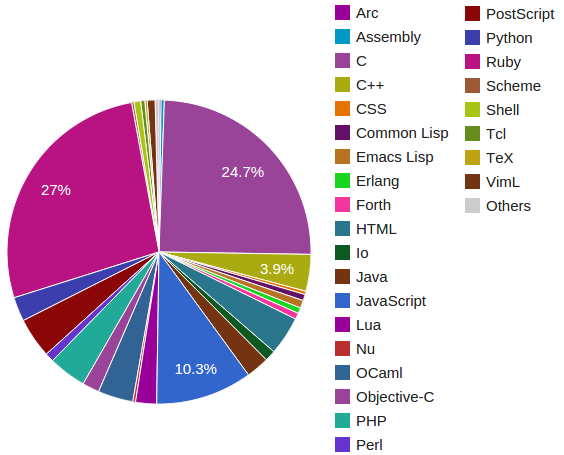
\includegraphics[width=0.8\linewidth]{images/sample1.png}
    \caption{First subset sample}
    \label{fig:sample1}
\end{figure}

\begin{figure}[h]
    \centering
    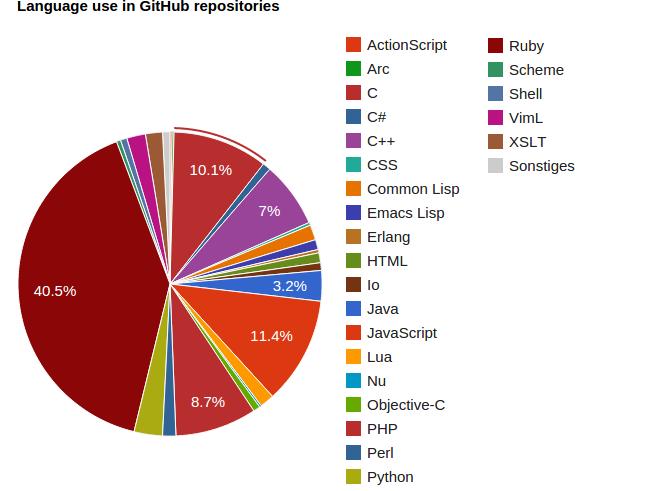
\includegraphics[width=0.8\linewidth]{images/sample2-since-4601.png}
    \caption{Second subset sample, repositories since 4601}
    \label{fig:sample2}
\end{figure}
\todo{2 more samples}
